% Exam Template for UMTYMP and Math Department courses
%
% Using Philip Hirschhorn's exam.cls: http://www-math.mit.edu/~psh/#ExamCls
%
% run pdflatex on a finished exam at least three times to do the grading table on front page.
%
%%%%%%%%%%%%%%%%%%%%%%%%%%%%%%%%%%%%%%%%%%%%%%%%%%%%%%%%%%%%%%%%%%%%%%%%%%%%%%%%%%%%%%%%%%%%%%

% These lines can probably stay unchanged, although you can remove the last
% two packages if you're not making pictures with tikz.
\documentclass[11pt]{exam}
\RequirePackage{amssymb, amsfonts, amsmath, latexsym, verbatim, xspace, setspace}
% \RequirePackage{tikz, pgflibraryplotmarks}

% By default LaTeX uses large margins.  This doesn't work well on exams; problems
% end up in the "middle" of the page, reducing the amount of space for students
% to work on them.
\usepackage[margin=1in]{geometry}

\usepackage[sc]{mathpazo}
\linespread{1.05}         % Palatino needs more leading (space between lines)
\usepackage[T1]{fontenc}

\usepackage{ulem}
\usepackage{graphicx}
\usepackage{enumitem}


% to generate random numbers
\usepackage{lcg}

% Here's where you edit the Class, Exam, Date, etc.
\newcommand{\class}{Class ID}
\newcommand{\term}{Spring 2018}
\newcommand{\examnum}{Midterm}
\newcommand{\examdate}{4/26/18}
\newcommand{\timelimit}{110 Minutes}

% For an exam, single spacing is most appropriate
\singlespacing

% For an exam, we generally want to turn off paragraph indentation
\parindent 0ex


\begin{document} 

% These commands set up the running header on the top of the exam pages
\pagestyle{head}
\firstpageheader{}{}{}
\runningheader{\class}{\examnum\ - Page \thepage\ of \numpages}{\examdate}
\runningheadrule

\begin{flushright}
\begin{tabular}{p{2.8in} r l}
\textbf{\class} & \textbf{Name (Print):} & \makebox[2in]{\hrulefill}\\
\textbf{\term} &&\\
\textbf{\examnum} &&\\
\textbf{\examdate} &&\\
\textbf{Time Limit: \timelimit} &&
% \textbf{Time Limit: \timelimit} & Teaching Assistant & \makebox[2in]{\hrulefill}
\end{tabular}\\
\end{flushright}
\rule[1ex]{\textwidth}{.1pt}


\begin{minipage}[t]{3.7in}
This exam contains \numpages\ pages (including this cover page) and
\numquestions\ problems.  Check to see if any pages are missing.  Put your initials
on the top of every page, in case the pages become separated.\\
\\

{\bf Do not write in the table to the right}.
\end{minipage}
\hfill
\begin{minipage}[t]{2.3in}
\vspace{0pt}
%\cellwidth{3em}
\gradetablestretch{2}
\vqword{Problem}
\addpoints % required here by exam.cls, even though questions haven't started yet.	
\gradetable[v]%[pages]  % Use [pages] to have grading table by page instead of question

\end{minipage}
\newpage % End of cover page

%%%%%%%%%%%%%%%%%%%%%%%%%%%%%%%%%%%%%%%%%%%%%%%%%%%%%%%%%%%%%%%%%%%%%%%%%%%%%%%%%%%%%
%
% See http://www-math.mit.edu/~psh/#ExamCls for full documentation, but the questions
% below give an idea of how to write questions [with parts] and have the points
% tracked automatically on the cover page.
%
%
%%%%%%%%%%%%%%%%%%%%%%%%%%%%%%%%%%%%%%%%%%%%%%%%%%%%%%%%%%%%%%%%%%%%%%%%%%%%%%%%%%%%%

\begin{questions}

%%%%%%%%%%%%%%%%%%%%%%%%%%%%%%
%%%%%%%%%%%%%%%%%%%%%%%%%%%%%%
\question[10]
{\bf The version of this figure WILL BE RANDOMIZED from exam version to exam version}

\begin{minipage}[l]{0.15\textwidth}
  \begin{enumerate}
 		\item \makebox[0.3in]{\hrulefill}
 		\item \makebox[0.3in]{\hrulefill}
 		\item \makebox[0.3in]{\hrulefill}
 		\item \makebox[0.3in]{\hrulefill}
 		\item \makebox[0.3in]{\hrulefill}
 		\item \makebox[0.3in]{\hrulefill}
	\end{enumerate}
\end{minipage}
\hfill
\begin{minipage}[r]{0.8\textwidth}
	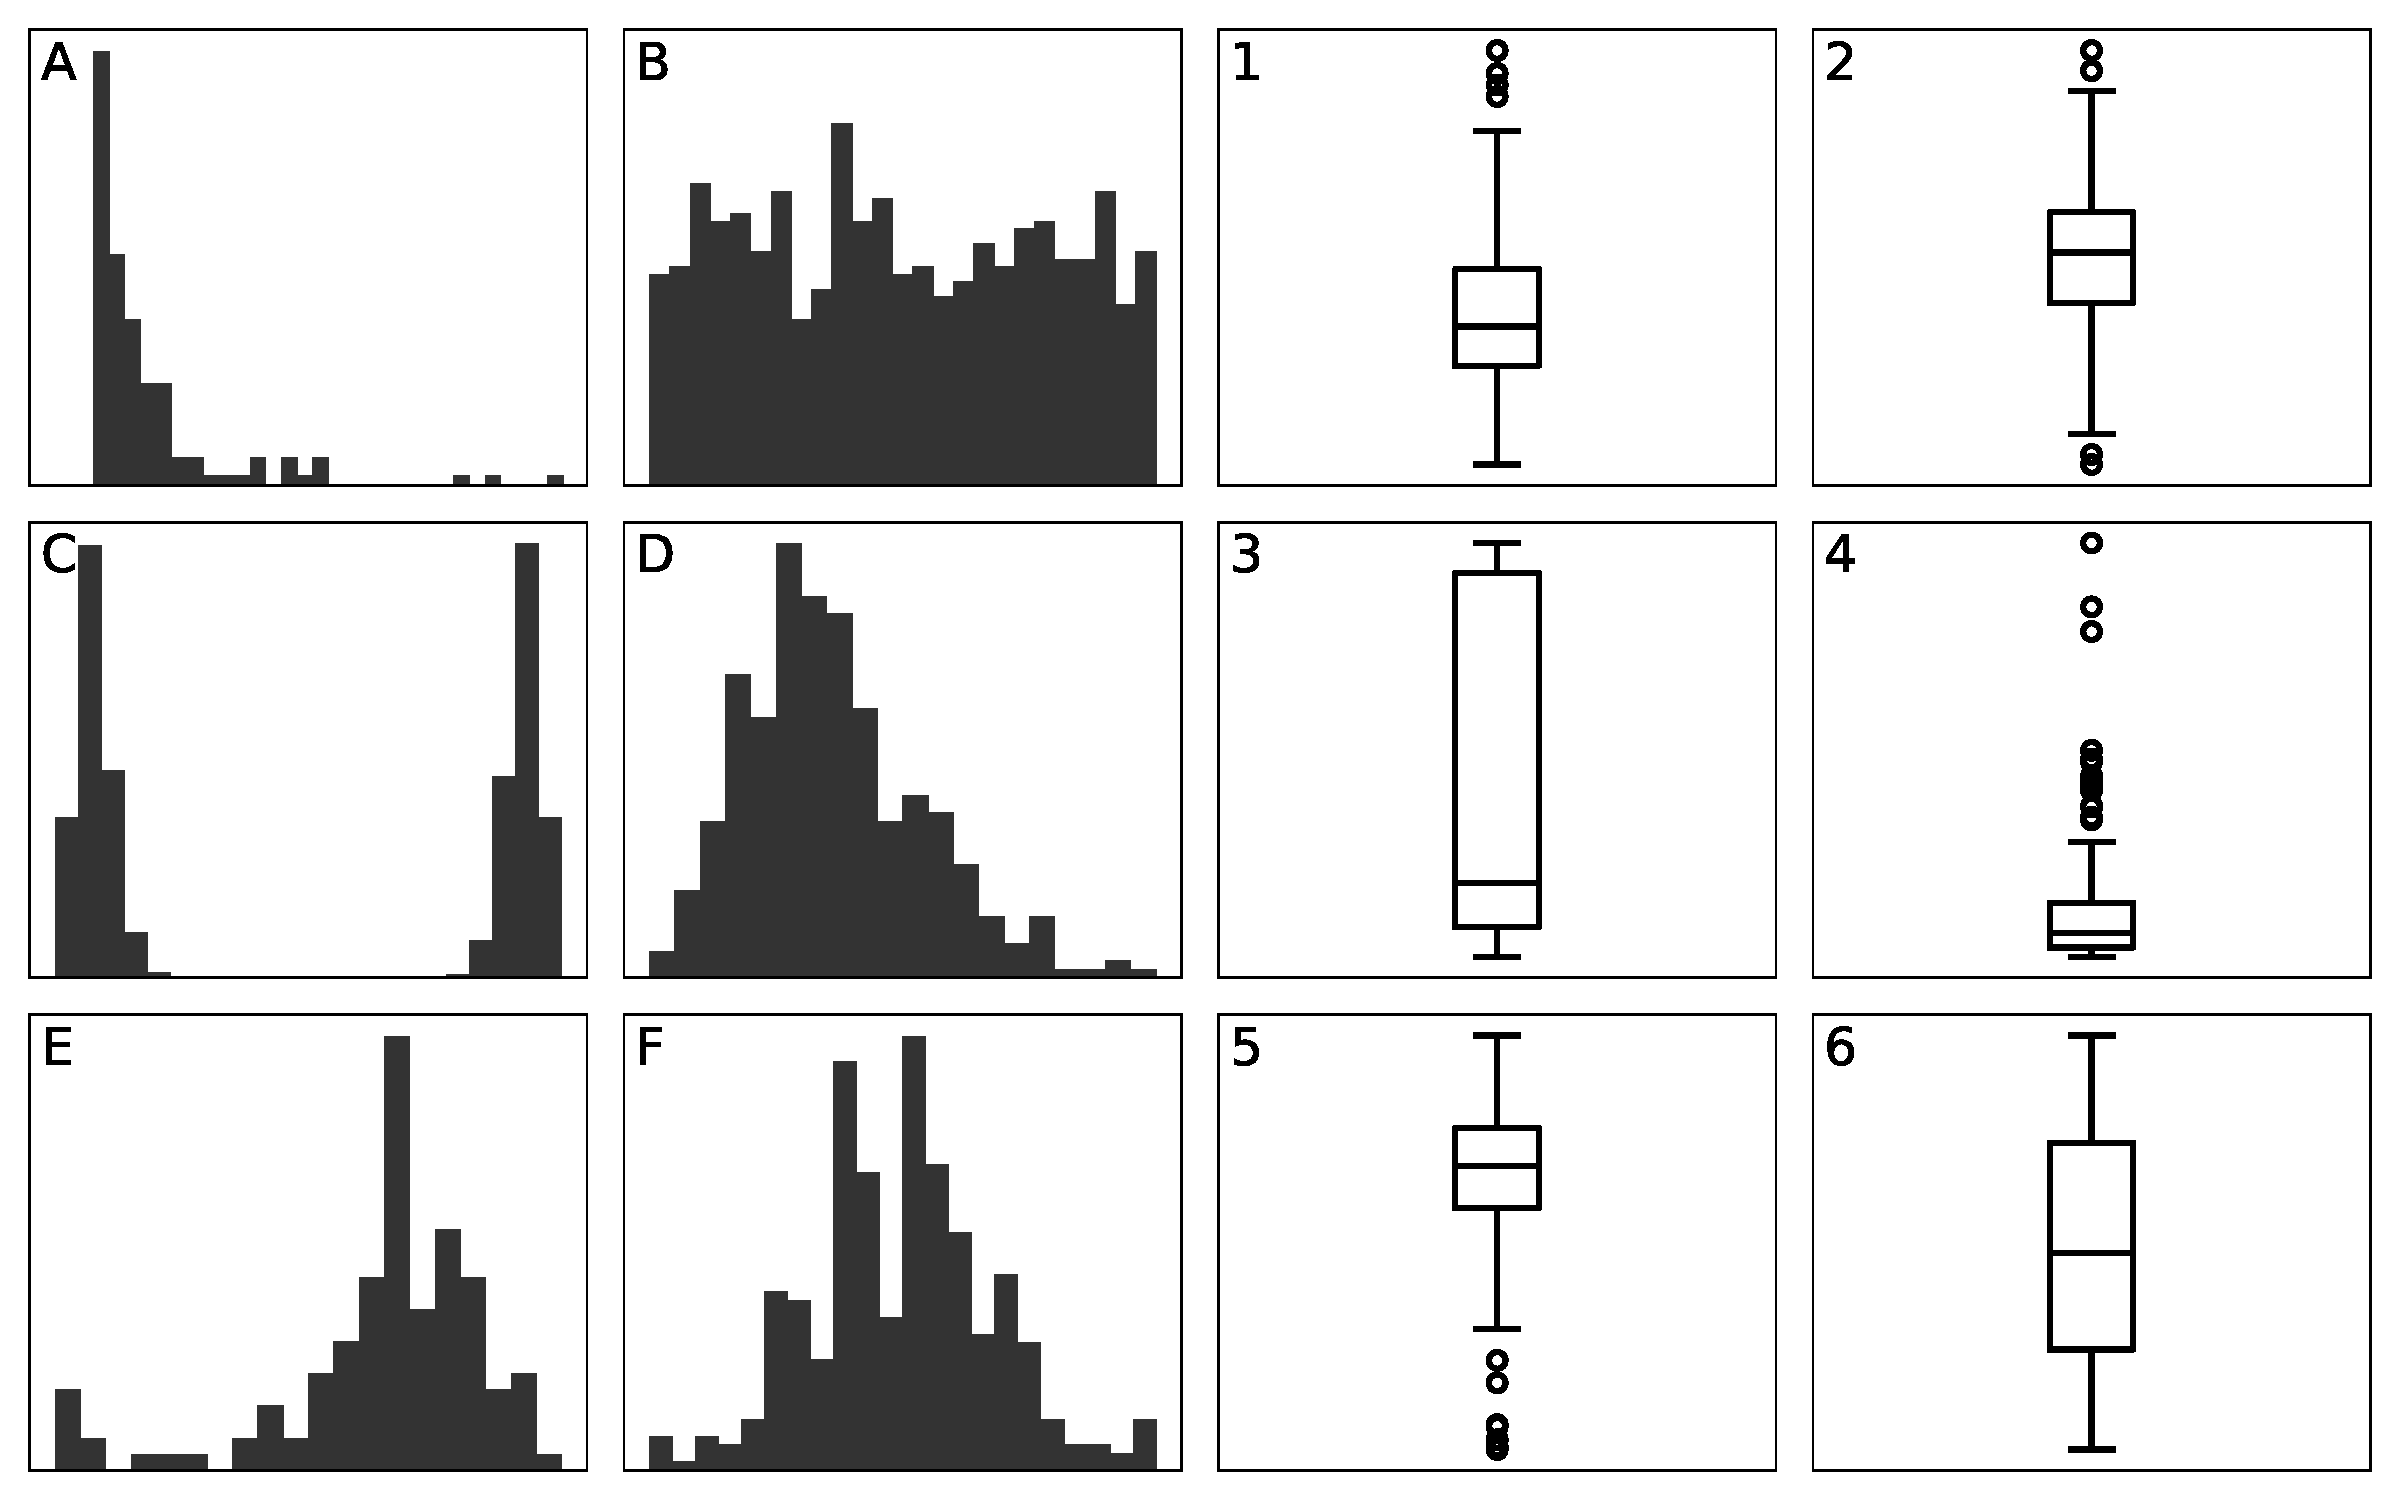
\includegraphics[width=\textwidth]{../figs/fig0.pdf}
\end{minipage}

{\bf The following three questions (a, b, c) concern the 6 rightmost panels in the figure above:}
\begin{enumerate}[label=\alph*.]
	\item What is the name of the type of summary plot used in those panels to represent the data? \makebox[1in]{\hrulefill}
	\item What are the 5 summary statistics that those plots display? \makebox[1in]{\hrulefill}, \makebox[1in]{\hrulefill}, \makebox[1in]{\hrulefill}, \makebox[1in]{\hrulefill}, \makebox[1in]{\hrulefill}
	\item What represent the circles in those plots? \makebox[1in]{\hrulefill}
\end{enumerate}
\vspace{2em}


\question[2]
{\bf Another question with something. The order of the item of this question won't be randomized.}	
	\begin{enumerate}
		\item item 1 with response to input: \makebox[1in]{\hrulefill}
 		\item item 2 with response to input: \makebox[1in]{\hrulefill}
	\end{enumerate}
\vspace{2em}


\question[2]
{\bf A multiple choice question. The order of the possible choices will be randomized from version to version}
	\begin{choices}
 		\choice A wrong answer
 		\CorrectChoice The correct answer
 		\choice A wrong answer
 		\choice A wrong answer
 		\choice A wrong answer
	\end{choices}
\vspace{2em}


\question[3]
{\bf The version of this figure WON'T BE RANDOMIZED from exam version to exam version. But the numbers in the table will be.}	
% set a counter for random numbers
\reinitrand[last=11, counter=num, quiet]

\begin{minipage}[l]{0.45\textwidth}
  \begin{tabular}{c|c|c|c|c|c}
    \rand\arabic{num}.\rand\arabic{num} & \rand\arabic{num}.\rand\arabic{num} & \rand\arabic{num}.\rand\arabic{num} & \rand\arabic{num}.\rand\arabic{num} & \rand\arabic{num}.\rand\arabic{num} & \rand\arabic{num}.\rand\arabic{num} \\ \hline
    \rand\arabic{num}.\rand\arabic{num} & \rand\arabic{num}.\rand\arabic{num} & \rand\arabic{num}.\rand\arabic{num} & \rand\arabic{num}.\rand\arabic{num} & \rand\arabic{num}.\rand\arabic{num} & \rand\arabic{num}.\rand\arabic{num} \\ \hline
    \rand\arabic{num}.\rand\arabic{num} & \rand\arabic{num}.\rand\arabic{num} & \rand\arabic{num}.\rand\arabic{num} & \rand\arabic{num}.\rand\arabic{num} & \rand\arabic{num}.\rand\arabic{num} & \rand\arabic{num}.\rand\arabic{num}
    
  \end{tabular}
\end{minipage}
\hfill
\begin{minipage}[r]{0.55\textwidth}
      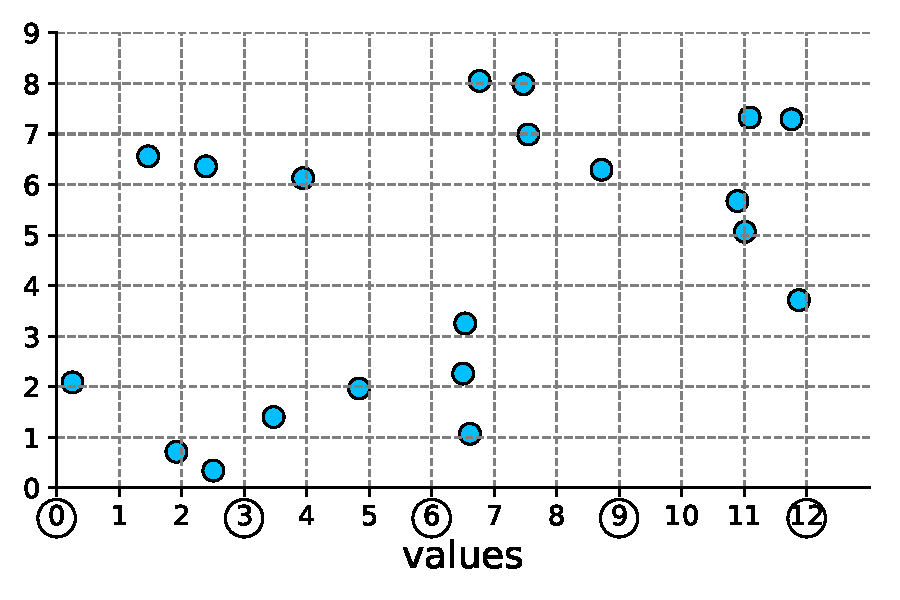
\includegraphics[width=\textwidth]{../figs/fig1.pdf}
\end{minipage}
\vspace{2em}


\question[2]
{\bf Another question with something. The order of the item of this question won't be randomized.}	
	\begin{enumerate}
		\item response 1
 		\item response 2
 		\item response 3
 		\item response 4
	\end{enumerate}
\vspace{2em}

\question[2]
{\bf A multiple choice question. The order of the possible choices will be randomized from version to version}
	\begin{choices}
 		\choice A wrong answer
 		\CorrectChoice The correct answer
 		\choice A wrong answer
	\end{choices}
\vspace{2em}


\end{questions}
\end{document}
